\chapter{Protocol Analyzer View}
\label{chapter:protoanalyzer}

Some filters for decoding packet-oriented data provide an alternate means of visualizing the decoded traffic.

The protocol analyzer view (Fig. \ref{proto-analyzer}) displays each packet in the history as a row in a list view. The
first column is always the timestamp of the packet; remaining columns vary depending on the particular filter in
question.

\begin{figure}[H]
\centering
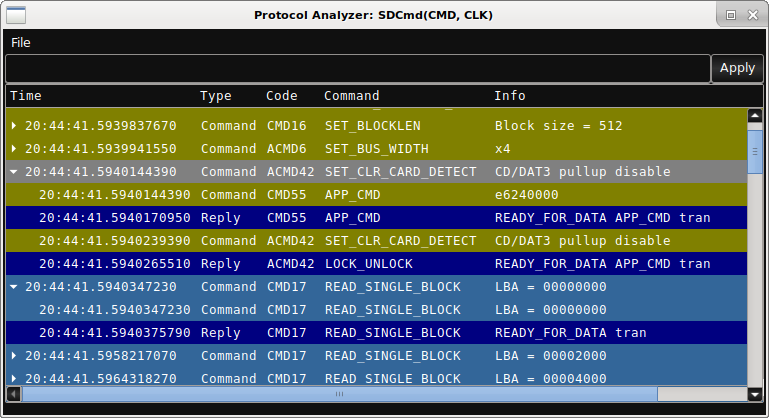
\includegraphics[width=14cm]{images/proto-analyzer.png}
\caption{Protocol analyzer view}
\label{proto-analyzer}
\end{figure}

If closed, the protocol analyzer view may be reopened by selecting the protocol of interest from the
\menustyle{Window / Analyzer} menu.

Many filters group related packets (request and reply, escape sequences, polling loops, etc) under a single heading to
enable easier navigation of large datasets. The tree expansion button at the left of the timestamp column may be used
to expand the event into its constituent packets.

\section{Cursor Interaction}

Clicking on a packet pauses acquisition, loads the relevant waveform from history if the packet is not in the current
waveform, and scrolls the waveform view containing the protocol decode to show the packet. If the packet fits entirely
within the view at the current zoom setting it is centered in the view; otherwise the beginning of the packet is placed
near the left edge of the viewport and the packet continues off the right edge.

If a vertical cursor (Sec. \ref{sec:cursors}) is active in the waveform area displaying the protocol decode, clicking
on a packet in the analyzer view moves the cursor to the start of the packet. Placing the cursor on a packet highlights
the corresponding row in the protocol analyzer.

\section{Packet Coloring}

Protocol packets are color coded according to the high-level function of the packet. The colors are configurable in
preferences; defaults are shown in the table below.

\begin{tabularx}{16cm}{llX}
\thickhline
\textbf{Color name} & \textbf{Use case} & \textbf{Default Color} \\
\thickhline
Command & Executing commands & \cellcolor{protocmd}\textcolor{white}{\#600050} \\
\thickhline
Control & Changing configuration & \cellcolor{protoctl}\textcolor{white}{\#808000} \\
\thickhline
Data read & Reading data & \cellcolor{protoread}\textcolor{white}{\#336699} \\
\thickhline
Data write & Writing data & \cellcolor{protowrite}\textcolor{white}{\#339966} \\
\thickhline
Error & Malformed, bad checksum & \cellcolor{protoerror}\textcolor{white}{\#ff0000} \\
\thickhline
Status & Status updates, flow control & \cellcolor{protostatus}\textcolor{white}{\#000080} \\
\thickhline
\end{tabularx}

\section{Filtering}

To ease analysis of large packet datasets, filters may be applied to the analyzer view by typing a filter expression
into the filter bar at the top of the window (Fig. \ref{proto-filter}), then pressing the ``Apply" button. A filter can
be removed by deleting the contents of the filter bar and pressing ``Apply".

\begin{figure}[H]
\centering
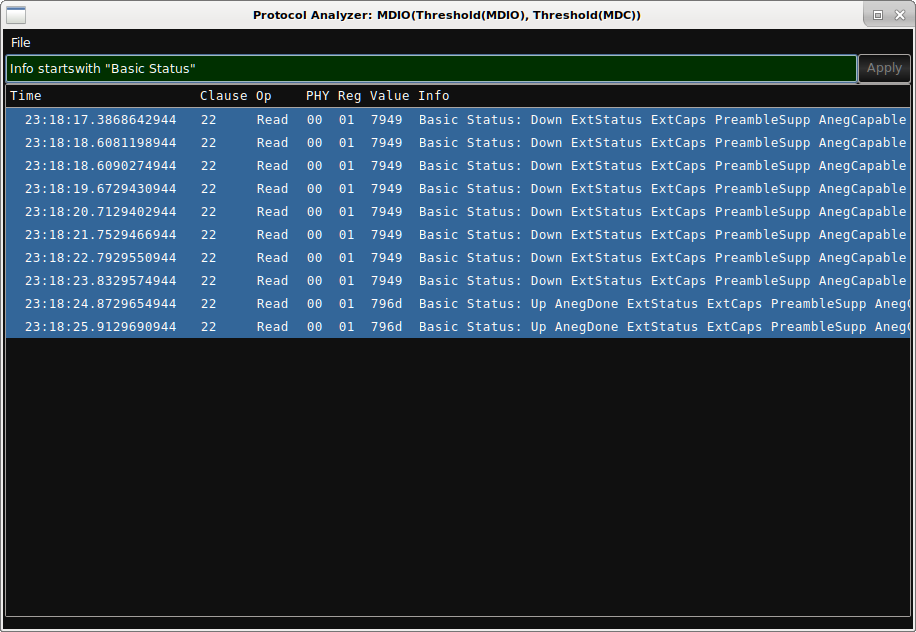
\includegraphics[width=14cm]{images/proto-filter.png}
\caption{Filtering protocol analyzer view}
\label{proto-filter}
\end{figure}

The basic format of a filter is (expression) (operator) (expression).

\subsection{Expressions}

An expression can be:
\begin{itemize}
\item A quoted string
\item A decimal number
\item A field identifier (such as \texttt{PHY} or \texttt{Reg}). Identifiers are case sensitive.
\item data[x], where x is an arbitrary numeric expression
\item A filter expression in parentheses. This expression must evaluate to boolean true or false. The unary ! operator
can be used to negate a parenthetical expression.
\end{itemize}

\subsection{Operators}

An operator can be:
\begin{itemize}
\item \texttt{==}: returns true if the left and right expression are equal
\item \texttt{!=}: returns true if the left and right expression are not equal
\item \texttt{||}: returns true if at least one of the left or right expression is true
\item \texttt{\&\&}: returns true if both the left and right expression is true
\item \texttt{startswith}: returns true if the right expression is a string which starts with the left expression
\item \texttt{contains}: returns true if the right expression is a string which contains the left expression
\end{itemize}

\subsection{Examples of filters}

\begin{lstlisting}[language=C]
Op == "Read"
Reg == "0f"
(Clause == 22) && (Info startswith "Basic Status")
\end{lstlisting}
